%; whizzy-master "main.tex"

\chapter{Tutorial}\label{chap:tutorial}

\begin{target}beginners.\end{target}

This chapter aims at helping a developer to write his first \framac plug-in. At
the end of the tutorial, any developer should be able to extend \framac with a
simple analysis available as a \framac plug-in. This chapter was written as a
step-by-step explanation on how to proceed towards this goal. It will get you
started, but it does not tell the whole story. You will get it with your own
experiments, and by reading the other chapters of this guide as needed.

First, Section~\ref{tut2:environment} describes how to quickly setup a
development environment for \framac.
Section~\ref{tut2:architecture} shows what a plug-in looks like. Then
Section~\ref{tut2:hello} explains the basis for writing a standard \framac
plug-in\index{Plug-in}, while Section \ref{tut2:cfg} details how to interact
with \framac and other plug-ins to implement analyzers of \C programs.

\section{Quick Setup of a Development Environment}\label{tut2:environment}

This setup is based on Emacs as the IDE, with OPAM for OCaml package
installation and Merlin for OCaml source code navigation.
Similar environments can be setup using other editors, such as Vim and
Sublime Text, but they are not detailed here; please refer to the Merlin
documentation for further details on how to setup other editors for OCaml
development.

\subsection{Emacs Configuration Files}

The \framac source distribution includes, in its \texttt{share} directory,
some \texttt{frama-c-*.el} files ({\em Emacs-lisp} scripts)
with default settings for an OCaml development environment based on
Emacs + OPAM + Merlin. To set it up, do the following:

\begin{enumerate}
\item Install Emacs, OPAM, and OPAM packages \textsf{merlin}, \textsf{tuareg}
  and \textsf{ocp-indent};
\item Copy \texttt{share/emacs/frama-c-*.el} to a directory in your Emacs load-path;
\item Add \texttt{(load-library "frama-c-recommended")} to your \texttt{.emacs}
  init file.
\end{enumerate}

For instance, run these commands (after having installed OPAM):

\begin{verbatim}
opam install merlin tuareg ocp-indent
mkdir ~/.emacs.d/frama-c
cp <path to frama-c sources>/share/emacs/frama-c-*.el ~/.emacs.d/frama-c/
\end{verbatim}

And then add this in the beginning of your \texttt{\textasciitilde/.emacs}:

\begin{verbatim}
(add-to-list 'load-path "~/.emacs.d/frama-c")
(load-library "frama-c-recommended")
\end{verbatim}

You can replace \texttt{frama-c-recommended} with \texttt{frama-c-dev} in the
above line. The former contains some extra, optional settings, while the latter
contains only the most important settings for OCaml development. We recommend
you review the definitions in \texttt{frama-c-recommended} and remove those you
find unnecessary.

\subsection{Quick Merlin guide}

Merlin\footnote{Merlin is available on Github
  (\url{https://github.com/the-lambda-church/merlin}) and as an OPAM package.}
is a tool for OCaml type information, source code navigation and
auto-completion.

Detailed instructions for using Merlin with Emacs are available at
\url{https://github.com/the-lambda-church/merlin/wiki/emacs-from-scratch}.

The \framac Makefile contains a target \textsf{merlin} that generates an
appropriate \texttt{.merlin} file to be used when editing \framac
\texttt{.ml/.mli} files. Run \texttt{make merlin} after compiling \framac,
and the generated \texttt{.merlin} file will be automatically used when opening 
\framac OCaml sources.

Here is a quick summary of the most useful commands when editing
\texttt{.ml/.mli} files:

\begin{itemize}
\item \texttt{Ctrl+c  Ctrl+t}: display type information
  (repeat it to further expand types)
\item \texttt{Ctrl+c  Ctrl+l}: jump to definition
  (for variables, types, modules, etc.)
\item \texttt{Ctrl+c  Ctrl+x}: jump to next error in current buffer
\end{itemize}

Merlin also includes an auto-complete feature. Check its website for
further documentation.

\section{What Does a Plug-in Look Like?}\label{tut2:architecture}
\index{Plug-in!Architecture}\index{Architecture!Plug-in}

Figure~\ref{fig:overview} shows how a plug-in can integrate with the \framac
platform. This tutorial focuses on specific parts of this figure.

\begin{figure}[ht]
\begin{center}
\newsavebox{\designbox}
\savebox{\designbox}{\begin{varwidth}{\textwidth}\centering Design\\(GUI extension point)\end{varwidth}}
\newlength{\designheight}
\setlength{\designheight}{\totalheightof{\usebox\designbox}}
\newsavebox{\captionbox}\savebox{\captionbox}{\textbf{Caption:}}
\newlength{\captionheight}\settototalheight{\captionheight}{\captionbox}
\begin{tikzpicture}[remember picture,txt/.style={inner xsep=3pt}]
  \node[inner sep=0pt] (implem) {
    \tikztitleboxbig{Plug-in\\implementation}{darkgreen}{
      \begin{tikz-vbox}{plugin-text}
        \node[on chain, draw, txt,minimum height=\designheight](register){Register};
        \node[on chain, draw, txt,minimum height=\designheight](options){Options};
        \node[on chain]{
          \begin{tikz-hbox}[every node/.style={minimum height=\designheight,minimum width=\designheight}]{etc-text}
            \node[draw, on chain]{};
            \node[on chain] {\ldots};
            \node[draw, on chain] {};
          \end{tikz-hbox}
        };
      \end{tikz-vbox}
    }
  };
  \node[anchor=south west,inner sep=0pt,xshift=\padding]
    at (implem.south east) (gui){
    \tikztitleboxbig{Plug-in GUI}{darkgreen}{
      \begin{tikz-hbox}{pluginguicontent}
        \begin{scope}[
          every node/.style={
            on chain,
            minimum width=\designheight,
            minimum height=\designheight}]
          \node[draw] {}; \node {\ldots}; \node[draw] {};
        \end{scope}
      \end{tikz-hbox}
    }
  };

  \coordinate[yshift=\padding] (makefile-se) at (gui.north east);
  \coordinate (makefile-nw) at (gui.west |- implem.north);
  \node[fill=palered, rounded corners=5pt,node font=\large,
        fit=(makefile-nw) (makefile-se),
        inner sep=0pt,draw]
        (makefile)
        {Makefile};

   \node[node font={\Large\bfseries},yshift=\padding,anchor=south]
   at ($(implem.north west)!0.5!(makefile.north east)$)
   (plugin-title)
   {Plug-in directory};
   \begin{scope}[on background layer]
     \node[fill=LightCyan, rounded corners=7pt,draw,
           fit=(implem) (gui) (makefile) (plugin-title), inner sep=\padding]
           (plugin-dir)
           {};
   \end{scope}

   \node[anchor=north,yshift=-\bigpadding,fill=Orange,draw]
   at (gui.south|-plugin-dir.south) (design) {\usebox\designbox};

   \node[anchor=north east,
         yshift=-\bigpadding-\captionheight]
   at (plugin-dir.east |- design.south) (registration) {registration points};
   \draw[Latex-] ($(registration.west)+(-\padding,0)$) -- +(-\bigpadding,0);

   \node[anchor=south east,xshift=-\padding] at (registration.north west)
   {\usebox{\captionbox}};

   \node[anchor=south,yshift=\bigpadding,fill=palered,draw,
   minimum height=1.5\designheight]
   at (plugin-dir.north -| gui.north) (makefile-dynamic) {Makefile.dynamic};

   \newlength{\kernelwidth}
   \setlength{\kernelwidth}{\widthof{Dynamic}}%TODO:compute dynamically
   \node[xshift=-\bigpadding,anchor=east] at (plugin-dir.west) {
     \begin{tikz-vbox}[every node/.style=
       {on chain,draw,fill=Orange,minimum height=\designheight,txt,
         minimum width=\kernelwidth}]
       {kernel}
       \node (db-main) {Db.Main};
       \node (dynamic) {Dynamic};
       \node (plugin)  {Plugin};
       \node (type)    {Type};
       \node (journal) {Journal};
       \node (project) {Project};
     \end{tikz-vbox}
   };

   \draw[-Latex] (makefile.north) -- (makefile-dynamic.south);
   \draw[-Latex] (gui.south) -- (design.north);
   \coordinate (main-pt) at ($(db-main.east)+(0.9\bigpadding,0)$);
   \draw (register.west) -| (main-pt);
   \draw[-Latex] (main-pt) -- (db-main.east);
   \draw[-Latex] (main-pt |- dynamic.east) -- (dynamic.east);

   \draw[-Latex] (options.west) -- (options.west -| main-pt)
                 -- +(-0.2\bigpadding,0) |- (plugin.east);

   \coordinate (implem-pt) at
   ($(options.west -| main-pt)+(-0.4\bigpadding,-\padding)$);
   \draw (implem-pt -| implem.west) -- (implem-pt);
   \draw[-Latex] (implem-pt) |- (type.east);
   \draw[-Latex] (implem-pt) |- (journal.east);
   \draw[-Latex] ($(plugin-dir.west |- implem-pt)+(0,-\padding)$)
      -- ($(implem-pt)+(0.2\bigpadding,-\padding)$) |- (project.east);

 \end{tikzpicture}
\end{center}
\scodeidx{Db}{Main}\codeidx{Dynamic}\codeidx{Plugin}
\codeidx{Project}\codeidx{Type}\codeidx{Journal}
\codeidx{Makefile.dynamic}\codeidx{Design}
\index{GUI}\index{Plug-in!GUI}
\caption{Plug-in Integration Overview.}\label{fig:overview}
\end{figure}

The implementation of the plug-in is provided inside a specific directory.
The plug-in registers with the \framac platform through
kernel-provided registration points. These
registrations are performed  through hooks\index{Hook} (by applying
a function or a functor). For instance,
the next section shows how to:
\begin{itemize}
\item extend the \framac entry point\index{Entry point} thanks to the function
  \texttt{Db.Main.extend}\sscodeidx{Db}{Main}{extend} if you want to run
  plug-in specific code whenever \framac is executed;
\item use specific plug-in services provided by the module
  \texttt{Plugin}\codeidx{Plugin}, such as adding a new \framac option.
\end{itemize}

\section{The Hello plug-in}\label{tut2:hello}

This simple plug-in explain how to make your plug-in interact basically
with several aspects of the \framac framework: registration, getting
command-line options, compilation and installation, console output,
testing, and documentation. (In case of difficulty, it is explained at
the end of this section how to generate the whole plug-in.)

\subsection{A Simple Script}\label{tut2:script}
\index{Plug-in!Script}

The easiest way to extend \framac is to write a simple script. A
simple 'Hello World' script consists of a single \ocaml file:

\listingname{./hello\_world.ml\footnotemark}
\ocamlinput{./tutorial/hello/generated/script/hello_world.ml}
\sscodeidx{Db}{Main}{extend} 

This script defines a simple function that writes a message to an
output file, then registers the function \texttt{run} as an entry point for the
script. \framac will call it among the other plug-in entry points if the script
is loaded.

The script is compiled, loaded and run with the command
\texttt{frama-c -load-script hello\_world.ml}. Executing this command
creates a \texttt{hello.out} file in the current directory.

\subsection{Registering a Script as a Plug-in}\label{tut2:plugin}
\index{Plug-in!Registration}

To make this script better integrated into \framac, its code must register
itself as a plug-in. Such a registration provides general services, such as
outputting on the \framac console, or extending \framac with new command-line
options.

Registering a plug-in is achieved through the use of the
\texttt{Plugin.Register} functor:

\listingname{./hello\_world.ml}
\ocamlinput{./tutorial/hello/generated/with_registration/hello_world.ml}
\sscodeidx{Db}{Main}{extend}
\scodeidx{Plugin}{Register}

The argument for this functor is a module with three values:
\begin{itemize}
\item \texttt{name} is an arbitrary, non-empty string containing the full name
  of the module.
\item \texttt{shortname} is a small string containing the short name of the
  module, usually used as a prefix for plug-in options. No space is allowed in
  that string.
\item \texttt{help} is a string containing free-form text, containing a
  description of the module.
\end{itemize}

Visible results of the registration include:
\begin{itemize}
\item ``hello world'' appears in the list of available plug-ins
  (consultable with \texttt{frama-c -load-script
    hello\_world.ml -plugins});
\item default options for the plug-in work, including the inline help
  (available with \texttt{frama-c -load-script
    hello\_world.ml -hello-help}).
\end{itemize}

\subsection{Displaying Messages}\label{tut2:messages}
\index{Plug-in!Messages}

The signature of the module \texttt{Self} obtained by applying
\texttt{Plugin.Register} is \texttt{General\_services}. One of these general
services is logging, \ie message display. In \framac, one should never attempt
to write messages directly to \texttt{stderr} or \texttt{stdout}: use the
general services instead\footnote{However writing to a new file using standard
  \ocaml primitives is OK.}.

\listingname{./hello\_world.ml}
\ocamlinput{./tutorial/hello/generated/with_log/hello_world.ml}
\sscodeidx{Db}{Main}{extend}
\scodeidx{Plugin}{Register}

Running this script yields the following output:
\begin{shell}
\$ frama-c -load-script hello_world.ml
[hello] Hello, world!
[hello] 11 * 5 = 55
\end{shell}

The \texttt{result} routine is the function to use to output results of your
plug-in. The \framac output routines takes the same arguments than the \caml
function \texttt{Format.printf}.

The function \texttt{feedback} outputs messages that show progress to the
user. In this example, we gave to feedback a log level of 2, because
we estimated that in most case the user is not interested in seeing
the progress of a fast operation (simple multiplication). The default
log level is 1, so by default this message is not displayed. To see
it, the verbosity of the \texttt{hello} plug-in must be increased:

\begin{shell}
\$ frama-c -load-script hello_world.ml -hello-verbose 2
[hello] Hello, world!
[hello] Computing the product of 11 and 5...
[hello] 11 * 5 = 55
\end{shell}

For a comprehensive list of the logging routines and options, see
Section~\ref{adv:log}.

\subsection{Adding Command Line Options}\label{tut2:basic-options}
\index{Plug-in!Command Line Options}\index{Command Line}

We now extend the \texttt{hello world} plug-in with new options.

If the plug-in is installed (with \texttt{make install}), it will be loaded and
executed on every invocation of \texttt{frama-c}, which is surely not what you
want. To avoid this behavior, we add a boolean option, set by default to false,
that conditionally enables the execution of the main function of the plug-in
(the usual convention for the name of the option is to take the short name of
the module with no suffix, \ie \texttt{-hello} in our case).

We also add another option, \texttt{-hello-output}, that takes a string
argument. When set, the hello message is displayed in the file given as
argument.

\listingname{./hello\_world.ml}
\ocamlinput{./tutorial/hello/generated/with_options/hello_world.ml}

Registering these new options is done by calling the \texttt{Self.False} and
\texttt{Self.String} functors, which respectively creates a new boolean option
whose default value is false and a new string option with a user-defined default
value (here \texttt{"-"}). The values of these options are obtained \via
\texttt{Enabled.get ()} and \texttt{Output\_file.get ()}. 

With this change, the hello message is displayed only if \framac is
executed with the \texttt{-hello} option.
\begin{shell}
\$ frama-c
\$ frama-c -load-script hello_world.ml -hello
[hello] Hello, world!
\$ frama-c -load-script hello_world.ml -hello -hello-output hello.out
\$ ls hello.out
hello.out
\end{shell}

These new options also appear in the inline help for the hello plug-in:
\begin{shell}
\$ frama-c -load-script hello_world.ml -hello-help
...
***** LIST OF AVAILABLE OPTIONS:

-hello              when on (off by default), output a warm welcome message
                    to the user (opposite option is -no-hello)
-hello-output <output-file>  file where the message is output (default:
                    output to the console)
...
\end{shell}


\subsection{Writing a Makefile}\label{tut2:basic-makefile}
\index{Plug-in!Makefile}

The use of \texttt{load-script} is ideal for small experimentations,
or when writing very specific extensions. When a plug-in becomes larger,
or more general-purpose, and must be split into several files, it is a
good idea to build and install it properly. \framac provides means to
simplify this through the use of \texttt{Makefile}s.

First, lets us create a \texttt{hello} directory that will contain all
of our plug-in files. We put \verb+hello_world.ml+ inside it, and then
create our \texttt{Makefile} there.

\subsubsection*{A simple Makefile}

% TODO: Recuperer toutes les informations du tutoriel 1

We write a simple \texttt{./Makefile} for our
\texttt{./hello\_world.ml} plug-in:

\listingname{./Makefile}
\codeidx{Makefile.dynamic}
\codeidx{FRAMAC\_SHARE}
\codeidx{PLUGIN\_CMO}
\codeidx{PLUGIN\_NAME}
\makefileinput{./tutorial/hello/generated/makefile_single/Makefile}

This \texttt{Makefile} sets some variables before including the generic
\texttt{Makefile.dynamic} which is installed within \framac. It may be
customized in several ways to help building a plug-in (see
Section~\ref{adv:dynamic-make} for details).

\begin{important}
  The name of each compilation unit (here \texttt{hello\_world}) must be
  different from the plug-in name set by the \texttt{Makefile} (here
  \texttt{Hello}), from any other plug-in names (\eg \texttt{value}\footnote{
    \texttt{value} is the technical plug-in name of the \texttt{Eva} plug-in})
    and from any other \framac kernel \caml files (\eg \texttt{plug-in}).
\end{important}

The plug-in also needs an interface file. Indeed, thanks to
\texttt{Makefile.dynamic}, each plug-in is packed into a single module
\texttt{\$(PLUGIN\_NAME)}\codeidx{PLUGIN\_NAME} (here \texttt{Hello}) which
needs an interface. Here we simply export an empty interface in order to hide
the whole implementation to other developers.

\listingname{./Hello.mli}
\ocamlinput{./tutorial/hello/src/Hello.mli}
\begin{important}
  Note the unusual capitalization of the filename \texttt{Hello.mli} which is
  required for compilation purposes.
\end{important}

Inside the plug-in's directory, run \texttt{make} to compile it. Note that the
compiled files are copied into a \texttt{top} (for {\em top-level}) subdirectory
(if our plug-in had GUI-dependent modules, they would be placed in a
\texttt{gui} subdirectory).
The module can then be loaded and executed by using
\texttt{frama-c -load-module top/Hello}.

Then run \texttt{make install} to install the plug-in (you need to have write
access to the \texttt{plugins} directory, located at the path given by the
command \texttt{frama-c-config -print-libpath}).

Just launch \texttt{frama-c} (without any option): the \texttt{Hello}
plug-in is now always loaded, without the need to pass other options to
the command line. Check it with the command \texttt{frama-c -hello-help}.

\subsubsection*{Splitting your source files}

Here is a slightly more complex example where the plug-in has been split into
several files. Usually plug-in registration through \texttt{Plugin.Register}
should be done at the bottom of the module hierarchy, while registration of the
run function through \texttt{Db.Main.extend} should be at the top, as in the
following example. The \texttt{PLUGIN\_CMO} variable must contain the list of
file names, in the correct \ocaml build order.

\listingname{./Makefile}
\codeidx{Makefile.dynamic}
\codeidx{FRAMAC\_SHARE}
\codeidx{PLUGIN\_CMO}
\codeidx{PLUGIN\_NAME}
\makefileinput{./tutorial/hello/generated/makefile_multiple/Makefile}

The three following files completely replace the \texttt{./hello\_world.ml}
from the previous section. Modules are directly called by their name in the
classical \ocaml way.

\listingname{./hello\_options.ml}
\ocamlinput{./tutorial/hello/generated/makefile_multiple/hello_options.ml}
\scodeidx{Plugin}{Register}

\listingname{./hello\_print.ml}
\ocamlinput{./tutorial/hello/generated/makefile_multiple/hello_print.ml}

\listingname{./hello\_run.ml}
\ocamlinput{./tutorial/hello/generated/makefile_multiple/hello_run.ml}
\sscodeidx{Db}{Main}{extend}

The plug-in can be tested again by running:

\begin{shell}
\$ make
\$ make install
<...>
\$ frama-c -hello -hello-output hello.out
\$ more hello.out
Hello, world!
\end{shell}

However, this does not consist in a proper test \emph{per se}. The next section
presents how to properly test plug-ins.

\subsection{Testing your Plug-in}\label{tut2:testing}
\index{Plug-in!Testing}\index{Test}

Frama-C supports non-regression testing of plug-ins. This is useful to check
that further plug-in modifications do not introduce new bugs. The tool allowing
to perform the tests is called \ptests\index{Ptests}.

To build these tests, the location of the subdirectories containing them must
be indicated in the \texttt{Makefile} through the variable
\texttt{PLUGIN\_TESTS\_DIRS}\codeidx{PLUGIN\_TESTS\_DIRS} set at
\texttt{hello} as this will be the name of the
subdirectory of \texttt{.tests/} where the plug-in's tests will be located:

\listingname{./Makefile}
\codeidx{Makefile.dynamic}
\codeidx{FRAMAC\_SHARE}
\codeidx{PLUGIN\_CMO}
\codeidx{PLUGIN\_NAME}
\codeidx{PLUGIN\_TESTS\_DIRS}
\makefileinput{./tutorial/hello/generated/with_test/Makefile}

This enables the creation of a
\texttt{./tests/ptests\_config} file holding the environement needed by
\ptests to run the plug-in's tests by running:
\begin{shell}
\$ mkdir tests
\$ make
<...>
Generating   tests/ptests_config
\end{shell}

For non-regression testing, the current behaviour of a program is taken as
the oracle against which future versions will be tested. In this tutorial, the
test will be about the correct \texttt{Hello, world!} output made by the option
\texttt{-hello} of the plug-in.

Each test directory must contain a
\texttt{run.config}\index{Test!Configuration}\index{Test!Header}
comment with the test directives\index{Test!Directive} and the C
source code used for the test.
(There are other ways to declare and control tests as developed
in Section~\ref{ptests:configuration}.)
For this tutorial, there will be no such source code. A file
\texttt{./tests/hello/hello\_test.c} is then created:

\listingname{./tests/hello/hello\_test.c}
\nscodeidx{Test!Directive}{OPT}
\lstinputlisting[style=c]{./tutorial/hello/generated/with_test/tests/hello/hello_test.c}

In this file, there is only one directive
\texttt{OPT: -hello}\nscodeidx{Test!Directive}{OPT} which requires
to run \framac on this test with the \texttt{-hello} option.
A look at Section~\ref{ptests:directives} gives you an idea of the kind of
directives which can be used to test plug-ins.

Once the \texttt{run.config} has been configured, it becomes possible to
get the output generated by the plug-in:
\begin{shell}[breaklines=true]
\$ ptests.opt -show
Env:
<...>
Command:
/usr/local/bin/frama-c.byte tests/hello/hello_test.c -check  -hello 2>tests/hello/result/hello_test.err.log >tests/hello/result/hello_test.res.log
[kernel] Parsing FRAMAC_SHARE/libc/__fc_builtin_for_normalization.i (no preprocessing)
[kernel] Parsing tests/hello/hello_test.c (with preprocessing)
[hello] Hello, world!
Env:
<...>
Command:
<...>
\end{shell}
The option \texttt{-show} runs the tests and shows the output
(but not their examination). Other options are detailed
in Section~\ref{ptests:options} to give a better idea of the
extent to which \ptests is configurable.
Under \texttt{Env} is displayed the context (coming from the file
\texttt{./hello/ptests\_config}).
Then, \texttt{Command} shows the executed command for this test case followed
by bash pipes to control the dataflow. (Note the \texttt{-hello}
option which has been passed to \framac as requested by \texttt{OPT: -hello}
in the \texttt{run.config}.)
Two outputs are considered as results for each test:
an \emph{error} output and a \emph{result} output.
These outputs are logged in the two following files:
\texttt{./tests/hello/result/hello\_test.err.log} and
\texttt{./tests/hello/result/hello\_test.res.log}.
The three lines beginning by \texttt{[kernel]} and \texttt{[hello]}
are the actual non-erroneous outputs made by \framac: two of them are generated
by the kernel (which could be muted by changing the verbosity) while the third
one is generated by our plug-in \texttt{Hello}. \texttt{Env} and
\texttt{Command} parts appear once again because some test strategies need it,
which is not the case in the simple setting of this tutorial.

Once you have verified the output is as expected, set it as an
oracle to be used for later non-regression tests by running:
\begin{shell}
\$ ptests.opt -update
\end{shell}
This command copies the two log files to
\texttt{./tests/hello/oracle/hello\_test.err.oracle} and
\texttt{./tests/hello/oracle/hello\_test.res.oracle}.

The setting of this test case is now finished.
Let's now assume the plug-in is later erroneously modified as follows:

\listingname{./hello\_run.ml}
\ocamlinput{./tutorial/hello/generated/with_test/hello_run_bug.ml}
\sscodeidx{Db}{Main}{extend}

where \texttt{Hello, world!} is incorrectly changed to \texttt{Hello world!}.
Running the command:
\begin{shell}[breaklines=true]
\$ make
<...>
\$ make tests
TESTING PLUG-IN Hello
% Dispatch finished, waiting for workers to complete
Env:
<...>
Command:
<...>
% Comparisons finished, waiting for diffs to complete
--- tests/hello/oracle/hello_test.res.oracle    2017-06-02 14:39:49.407624816 +0200
+++ tests/hello/result/hello_test.res.log       2017-06-02 14:40:03.483624679 +0200
@@ -1,3 +1,3 @@
 [kernel] Parsing FRAMAC_SHARE/libc/__fc_builtin_for_normalization.i (no preprocessing)
 [kernel] Parsing tests/hello/hello_test.c (with preprocessing)
-[hello] Hello, world!
+[hello] Hello world!
% Diffs finished. Summary:
Run = 1
Ok   = 1 of 2
Time = 0.380000 s.
real 0.45
user 0.38
sys 0.03
\end{shell}
displays the differences (à la \texttt{diff}) between the current executions
and the saved oracles. Here the diff clearly shows that the only difference is
the missing comma in the generated message due to our (erroneous) modification.
One test is marked as being successful: that is the test comparing
\texttt{stderr} (which contains an empty string). After fixing the \ocaml code,
running \texttt{make \&\& make tests} again shows that all test cases are
successful.

You may use other \framac's plug-ins as examples of how to integrate a
plug-in with \ptests. Small plug-ins such as \texttt{Report} and
\texttt{Variadic} are good examples (see directories
\texttt{src/plugins/report/tests/} and \texttt{src/plugins/variadic/tests/}).
Please note \framac offers no particular support for other kinds of testing
purposes, such as test-driven development (TDD)\footnote{For the purpose of
driving the development of a plug-in, one should have to manually create
\texttt{./tests/*/oracle/*.err.oracle} and
\texttt{./tests/*/oracle/*.res.oracle} files for example.} for instance.
Additional information about plug-in testing is available in
Sections~\ref{adv:ptests} and~\ref{sec:ptests}.

\subsection{Documenting your Source Code}
\label{tut2:doc}
\index{Plug-in!Documentation}

\framac automatically generates the documentation of plug-ins when the command
\texttt{make doc} is run\footnote{Frama-C kernel needs to have been
installed with code documentation support. If this was not the case, you can
run \texttt{make doc install-doc-code} in Frama-C's main directory as hinted
by the error message appearing in the terminal before trying again to generate
the documentation of the plug-in.}. This relies on \ocamldoc and
requires the plug-in to be documented following the \ocamldoc guidelines
(please refer to the corresponding chapter in \cite{caml}).

We show here how the Hello plug-in could be slightly documented and use
\ocamldoc features such as @-tags and cross references:

\listingname{./hello\_options.ml}
\ocamlinput{./tutorial/hello/generated/with_doc/hello_options.ml}
\scodeidx{Plugin}{Register}

\listingname{./hello\_print.ml}
\ocamlinput{./tutorial/hello/generated/with_doc/hello_print.ml}

\listingname{./hello\_run.ml}
\ocamlinput{./tutorial/hello/generated/with_doc/hello_run.ml}
\sscodeidx{Db}{Main}{extend}

The documentation files of the plug-in are added to
\texttt{./doc/code/} and the link to this
is added to the plug-ins index file
\texttt{./doc/code/index.html}.

This simple tutorial now comes to its end. It focused on the standard features of
architectures and interfaces of \framac plug-ins. A companion archive
\texttt{hello.tar.gz} is available in the download section of the \framac
website\footnote{The direct link is: \url{http://frama-c.com/download.html}.}.
The next tutorial will make you dive in \C analysis.

%%%%%%%%%%%%%%%%%%%%%%%%%%%%%%%%%%%%%%%%%%%%%%%%%%%%%%%%%%%%%%%%%%%%%%%%%%%%%%%%

\section{The ViewCfg plug-in}\label{tut2:cfg}

In this section, we create a new ViewCfg plug-in that computes the control
flow graph of a function and outputs it in the \dottool format. Through its
implementation, we explain some of \framac APIs such as how to visit
an AST\footnote{Abstract Syntax Tree}, to hook a plug-in, to interface
a plug-in with other plug-ins, to extend the
GUI\footnote{Graphical User Interface}, to make a plug-in usable by
others, to make write a plug-in into the journal, to configure a script,
and to make a plug-in usable in a multi-projects setting.

This section assumes the reader is already familiar with the basics of plug-ins
for \framac as covered by the Hello plug-in in the previous
section.

\subsection{Visiting the AST}\label{tut2:visitor}
\index{Visitor}

Writing an analysis for \C programs is the primary purpose of a \framac
plug-in. That usually requires to visit the AST to compute information for some
\C constructs. There are two different ways of doing that in \framac:
\begin{itemize}
\item through a direct recursive descent; or
\item by using the \framac visitor.
\end{itemize}
The first case is usually better if you have to compute information for most \C
constructs, while the latter is better if only few \C constructs are interesting
or if you have to write a program transformation. Of course, it is also possible
to combine both ways to tune it to specific needs.

\subsubsection*{Pretty-printing with direct recursive descent}

Frama-C already has a function to pretty-print statements (namely
\texttt{Printer.pp\_stmt}\scodeidx{Printer\_api}{S.pp\_stmt}), but it is not suitable
for us, as it will recursively print substatements of compound statements
(blocks, if, while, ...) while we only want to pretty print the node representing the
current statement: substatements will be represented by other nodes. Thus we
will use the following small function:
\ocamlinput{./tutorial/viewcfg/src/print_stmt.ml}
\sscodeidx{Cil\_types}{stmtkind}{Instr}
\sscodeidx{Cil\_types}{stmtkind}{Return}
\sscodeidx{Cil\_types}{stmtkind}{Goto}
\sscodeidx{Cil\_types}{stmtkind}{Break}
\sscodeidx{Cil\_types}{stmtkind}{Continue}
\sscodeidx{Cil\_types}{stmtkind}{If}
\sscodeidx{Cil\_types}{stmtkind}{Switch}
\sscodeidx{Cil\_types}{stmtkind}{Loop}
\sscodeidx{Cil\_types}{stmtkind}{Block}
\sscodeidx{Cil\_types}{stmtkind}{UnspecifiedSequence}
\sscodeidx{Cil\_types}{stmtkind}{TryFinally}
\sscodeidx{Cil\_types}{stmtkind}{TryExcept}
\scodeidx{Printer\_api}{S.pp\_instr}
\scodeidx{Printer\_api}{S.pp\_exp}

The \texttt{Cil\_types} module contains the definition of the AST of a \C
program, like constructors \texttt{Cil\_types.Instr},
\texttt{Cil\_types.Return}, and so on which are of type
\texttt{Cil\_types.stmtkind}. The \texttt{Printer} module contains
functions that prints the different Cil types. The documentation of these module
is available on the \framac website\footnote{From
  \url{http://frama-c.com/download.html}.}, or by typing \texttt{make doc} in
the \framac source distribution.

\subsubsection*{Creating the graphs with a visitor}

In order to create our output, we must make a pass through the whole
AST. An easy way to do that is to use \framac visitor mechanism. A
visitor is a class with one method per type of the AST, whose default
behavior is to just call the method corresponding to each of its
children. By inheriting from the visitor, and redefining some of the
methods, one can perform actions on selected parts of the AST, without
the need to traverse the AST explicitly.

\ocamlinput{./tutorial/viewcfg/src/print_cfg_begin.ml}
\scodeidx{Visitor}{frama\_c\_inplace}

Here we used the so-called ``in place'' visitor, which should be used for
read-only access to the AST. When performing code transformations, a
``copy'' visitor should be used, that creates a new project (see
section~\ref{sec:visitors-projects}).

There are three kinds of nodes where we have something to do. First,
at the file level, we create the whole graph structure.

\ocamlinput{./tutorial/viewcfg/src/print_cfg_vfile.ml}
\sscodeidx{Cil}{visitAction}{DoChildrenPost}
\sscodeidx{Cil}{cilVisitor}{vfile}

\texttt{Cil.DoChildrenPost} is one of the possible
\texttt{visitAction}, that tells the visitor what to do after the
function is executed. With \texttt{DoChildrenPost func}, the \texttt{func}
argument is called once the children have been executed: here we close the
parenthesis once that all functions have been printed in the file.

Then, for each function, we encapsulate the CFG in a subgraph, and do
nothing for the other globals.

\ocamlinput{./tutorial/viewcfg/src/print_cfg_vglob.ml}
\sscodeidx{Cil}{visitAction}{DoChildrenPost}
\sscodeidx{Cil}{visitAction}{SkipChildren}
\sscodeidx{Visitor}{frama\_c\_visitor}{vglob\_aux}
\scodeidx{Cil\_types}{GFun}
\scodeidx{Printer\_api}{S.pp\_varinfo}

\texttt{Cil.SkipChildren} tells the visitor not to visit the children
nodes, which makes it more efficient\footnote{In a copying visitor,
\texttt{Cil.JustCopy}\sscodeidx{Cil}{visitAction}{JustCopy}
should have been used instead.}.

Last, for each statement, we create a node in the graph, and create
the edges toward its successors:

\ocamlinput{./tutorial/viewcfg/src/print_cfg_vstmt_aux_novalue.ml}
\sscodeidx{Cil}{visitAction}{DoChildren}
\sscodeidx{Visitor}{frama\_c\_visitor}{vstmt\_aux}

This code could be optimized, for instance by replacing the final
\texttt{DoChildren} by \texttt{SkipChildren} for statements that
cannot contain other statements, like \texttt{Instr}, and avoid
visiting the expressions.

Finally we close the \texttt{object} definition:
\ocamlinput{./tutorial/viewcfg/src/print_cfg_end.ml}

\subsubsection*{Hooking into \framac}

It just remains to hook this script into \framac.

\ocamlinput{./tutorial/viewcfg/src/extend_with_simple_run.ml}

Assuming the script is called \texttt{cfg\_print.ml}, it can then be run with:
\begin{shell}
  frama-c -load-script cfg_print.ml [other_options] file.c [file2.c] 
\end{shell}

And the graph can be visualized with 
\begin{shell}
  dotty cfg.out
\end{shell}

This produces a graph like in Figure~\ref{fig:tut:basiccfg}

\begin{figure}[htbp]
  \centering
  \begin{minipage}[h]{0.45\linewidth}
  \listingname{test.c}
  \cinput{./tutorial/viewcfg/tests/test.c}
  \end{minipage}%
  \begin{minipage}[h]{0.4\linewidth}
    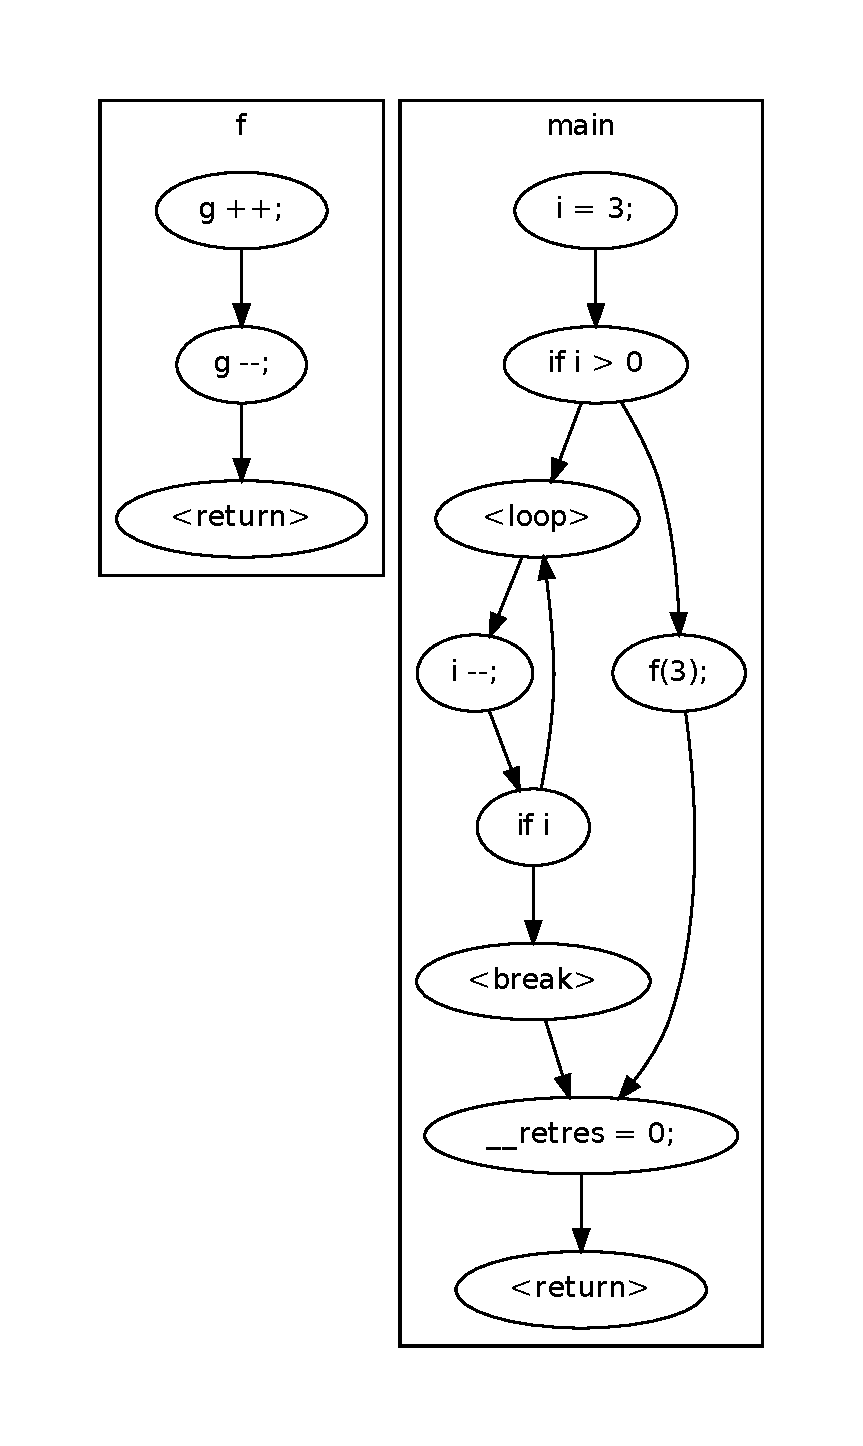
\includegraphics[width=\textwidth]{./tutorial/viewcfg/pdfs/cfg.pdf}
  \end{minipage}

  \caption{Control flow graph for file test.c.}
  \label{fig:tut:basiccfg}
\end{figure}

\subsubsection*{Further improvements}

There are many possible enhancements to this code:

\begin{itemize}
\item There is a bug when trying to print statements that contain
  strings (such as \verb|printf("Hello\n")| such statements must be
  protected using the \verb|"%S"| Format directive;
\item The script could be transformed into a regular plug-in, by
  registering into \framac, and taking options from the command line;
  for instance to compute the control flow graph of a single function
  given as an argument;
\item The graphs could be fancier, in particular by distinguishing
  between branching nodes and plain ones, or showing exit of blocks as
  well as their beginning; or linking a call with the called function.
\end{itemize}

We will concentrate on another extension, which is to reuse the
analysis of the \texttt{value} \framac plug-in to color unreachable
nodes.
To do so, because we will combine different plug-ins, we need to ensure their
correct ordering. This requires the definition of some command-line options.

\subsection{Plug-In registration and command-line options}\label{tut2:options}
\index{Plug-in!Command Line Options}\index{Command Line}

We have already seen how to register options in the previous ``Hello'' tutorial.
We now apply these principles to the ViewCfg plug-in.

\ocamlinput{./tutorial/viewcfg/src/register_and_options.ml}
\scodeidx{Plugin}{Register}
\ocamlinput{./tutorial/viewcfg/src/extend_with_run_with_options.ml}
\scodeidx{Visitor}{visitFramacFileSameGlobals}
\scodeidx{Ast}{get}

We added two options, \texttt{-cfg} to compute the CFG
conditionally (important for ordering plug-in executions),
and \texttt{-cfg-output} to choose the output file.

An interesting addition would be a \texttt{-cfg-target} option,
which would take a set of files or functions whose CFG would be
computed, using the \texttt{Self.Kernel\_function\_set} functor. Depending on
the targets, visiting the AST would have different starting points.
This is left as an exercise for the reader.

Another interesting exercise is to solve the following problem.
Currently, the complete CFG for the whole application is computed in
each \framac step, \ie executing \texttt{frama-c test.c -cfg
  -then -report} would compute the CFG twice. Indeed, the
\texttt{-cfg} option sets \texttt{Enabled} to true, and the
\texttt{run} function is executed once per task. To solve this
problem, one has to create a boolean state to remember that the plug-in
has already been executed. The \texttt{apply\_once} function in the
\texttt{State\_builder} module helps dealing with this issue (reading
the section~\ref{tut2:project-and-state} of this tutorial and
section~\ref{adv:project} of this manual should help you understand the
underlying notion of states).

With these command-line options, we can properly interface our ViewCfg plug-in
with the \texttt{value} plug-in.

\subsection{Interfacing with a kernel-integrated plug-in}

Kernel-integrated plug-ins, such as \texttt{value}, use a special mechanism
to statically register their APIs for other plug-ins that wish to access them.
This mechanism is the \texttt{Db} module of the \framac kernel,
the entry point for all kernel-integrated plug-ins. By using the functions
exported through the \texttt{Db.Value} module, our plug-in will obtain
reachability information computed by \texttt{value}.

The code modification we propose is to color in pink the nodes guaranteed to
be unreachable by the value analysis. For this purpose, we change the
\texttt{vstmt\_aux} method in the visitor:

\ocamlinput{./tutorial/viewcfg/src/print_cfg_vstmt_aux_value.ml}
\sscodeidx{Db}{Value}{is\_computed}
\sscodeidx{Db}{Value}{get\_stmt\_state}
\sscodeidx{Db}{Value}{is\_reachable}
\sscodeidx{Cil}{visitAction}{DoChildren}
\sscodeidx{Visitor}{frama\_c\_visitor}{vstmt\_aux}

This code fills the nodes with green if the node may be
reachable, and in pink if the node is guaranteed not to be
reachable; but only if the value analysis was previously computed. 

To test this code, frama-c should be launched with:
\begin{shell}
  frama-c test.c -load-script cfg_print.ml -val -then -cfg && dotty cfg.out
\end{shell}

Note that the relative order of the parameters \texttt{-load-script} and
\texttt{-val} in this example is not relevant
(see Section~\ref{adv:init} for details).
However, it is important to ensure that \texttt{-cfg} is separated from
\texttt{-val} by a \texttt{-then}; otherwise, it is not guaranteed that
the \texttt{value} plug-in will run before the ViewCfg plug-in, which might
lead to a non-colored graph in some cases, and colored in others.

The resulting graph is shown in Figure~\ref{fig:tut:coloredcfg}.

\begin{figure}[htbp]
  \centering
  \begin{minipage}[h]{0.45\linewidth}
  \listingname{test.c}
  \cinput{./tutorial/viewcfg/tests/test.c}
  \end{minipage}%
  \begin{minipage}[h]{0.4\linewidth}
    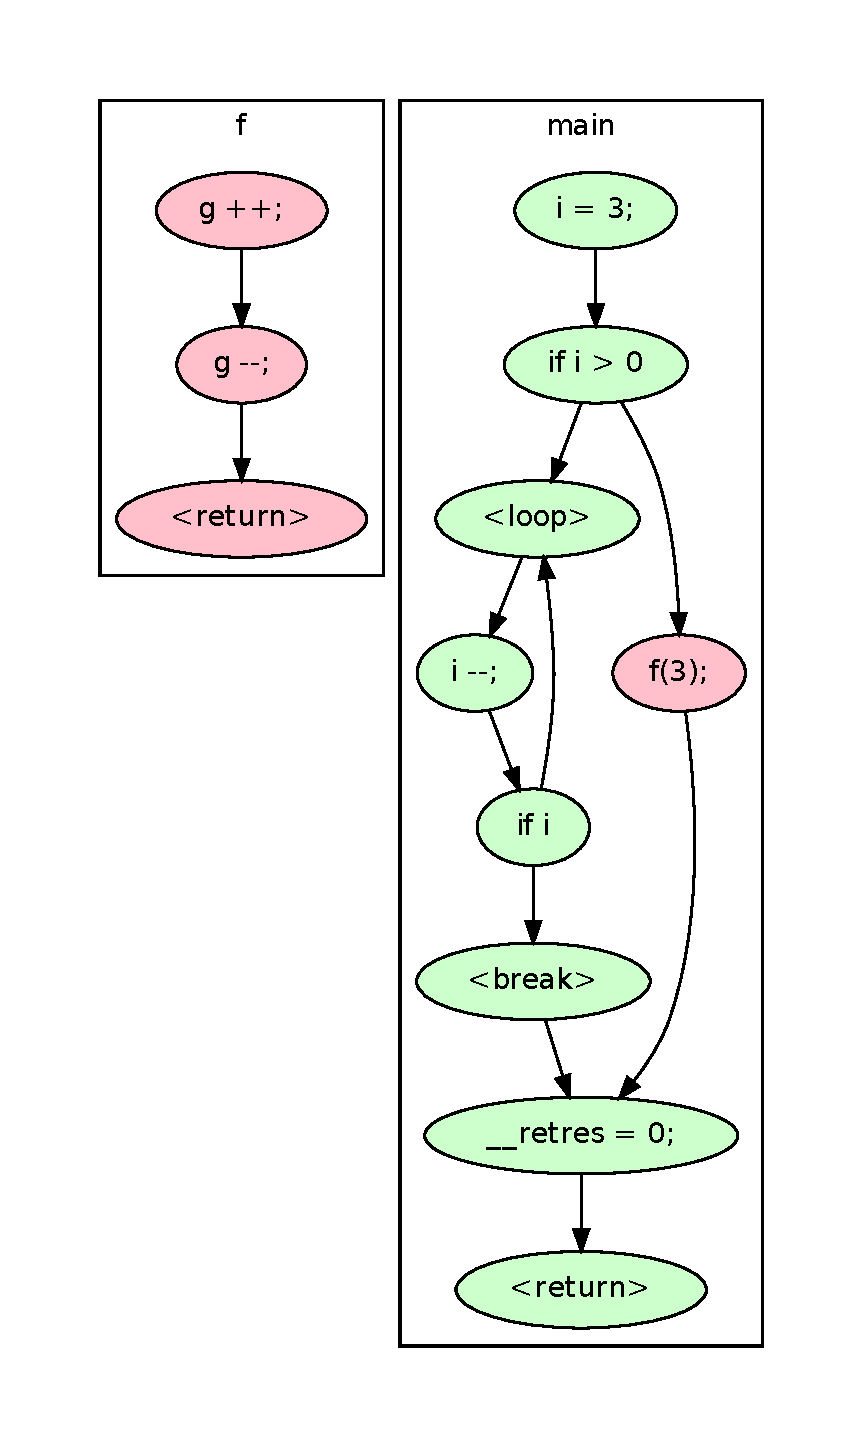
\includegraphics[width=\textwidth]{./tutorial/viewcfg/pdfs/cfg_colored.pdf}
  \end{minipage}
  \caption{Control flow graph colored with reachability information.}
  \label{fig:tut:coloredcfg}
\end{figure}

\subsection{Extending the Frama-C GUI}
\label{tut2:gui}
\index{Plug-in!GUI}

In this section, we will extend our plug-in so that the control flow
graph can be displayed interactively. For that, we will extend the \framac GUI
so that when you right-click on a function in the code, a new ``Show
CFG'' item appears, that displays the control flow graph of the
function in a dialog box. This is achieved just by appending the following
pieces of code at the end of the \texttt{cfg\_print.ml} file.

Currently, we used a visitor that outputs a \dottool file with the CFG of
all functions of all files. We use \texttt{dump\_function} to output
the CFG of a single function instead.

\ocamlinput{./tutorial/viewcfg/src/dump_function.ml}

We reused the \texttt{print\_cfg} visitor, but we selected a different
starting point. The argument \texttt{fundec} gets type
\texttt{Cil\_types.fundec}\scodeidx{Cil\_types}{fundec}, which is the CIL type
representing a function definition.

Now we write the GUI extension code:

\ocamlinput{./tutorial/viewcfg/src/gui.ml}
\scodeidx{Pretty\_source}{PVDecl}
\sscodeidx{Globals}{Functions}{get}
\scodeidx{Kernel\_function}{get\_definition}
\scodeidx{Gtk\_helper}{graph\_window}
\scodeidx{Design}{register\_extension}
\sscodeidx{Design}{main\_window\_extension\_points}{register\_source\_selector}

Let us explain this code from the end. \texttt{Design.register\_extension} is
the entry point for extending the GUI. Its argument is a function which takes as
argument an object corresponding to the main window of the \framac GUI. This
object provides access to the main widgets of the window, and several
extension points.

Here we have implemented a single extension, the ``source selector'',
that allows to add entries to menu obtained when right-clicking on the
source. This is implemented by the \texttt{cfg\_selector} function.

This function takes a \texttt{localizable} argument, which gives information on
where the user clicks on the source. Here we do something only if the user
clicks on the declaration of a variable whose type is a function (\ie when the
user clicked on a function declaration or definition).  In that case, we add an
item to the popup menu, that calls the \texttt{callback} function if
clicked. The \texttt{callback} function calls a \framac GUI function that
displays a graph from \dottool printing functions. It uses several important \framac
APIs: \texttt{Globals} and \texttt{Kernel\_function}, which contain several
functions for manipulating globals and functions.

Note that this GUI extension could also have been done through a script
(instead of a plug-in), but it would have been less than ideal.
In particular, the GUI \ocaml modules are available only when a script
is loaded with \texttt{frama-c-gui}, and not when loaded with
\texttt{frama-c}. When the user wants to view the CFG from the GUI,
outputting the CFG of all functions in \texttt{cfg.out} is useless.
A better architectural solution is to split our plug-in in several files,
with its own Makefile, to better manage its functionalities.

\subsection{Splitting files and writing a Makefile}\label{tut2:makefile}
\index{Plug-in!Makefile}

The \framac plug-in development environment allows to split GUI-related
and non-GUI related modules, so that GUI-related modules are loaded
and run only if \framac is executed with \texttt{frama-c-gui}. This
requires splitting the module into several files. We choose the
following architecture:

\begin{itemize}
\item \texttt{cfg\_options.ml} implements plug-in registration and
  configuration options;
\item \texttt{cfg\_core.ml} implements the main functions for
  computing the CFG;
\item \texttt{cfg\_register.ml} implements ``global'' computation of
  the CFG using the \texttt{-cfg} option, and hooking into the \framac
  main loop;
\item \texttt{cfg\_gui.ml} implements GUI registration.
\end{itemize}

Dependencies between the modules\footnote{This graphic is generated in
  file \texttt{doc/code/modules.dot} after running \texttt{make doc}.}
is presented on Figure \ref{fig:tut:cfgarchitecture}.

\begin{figure}[htbp]
  \centering
    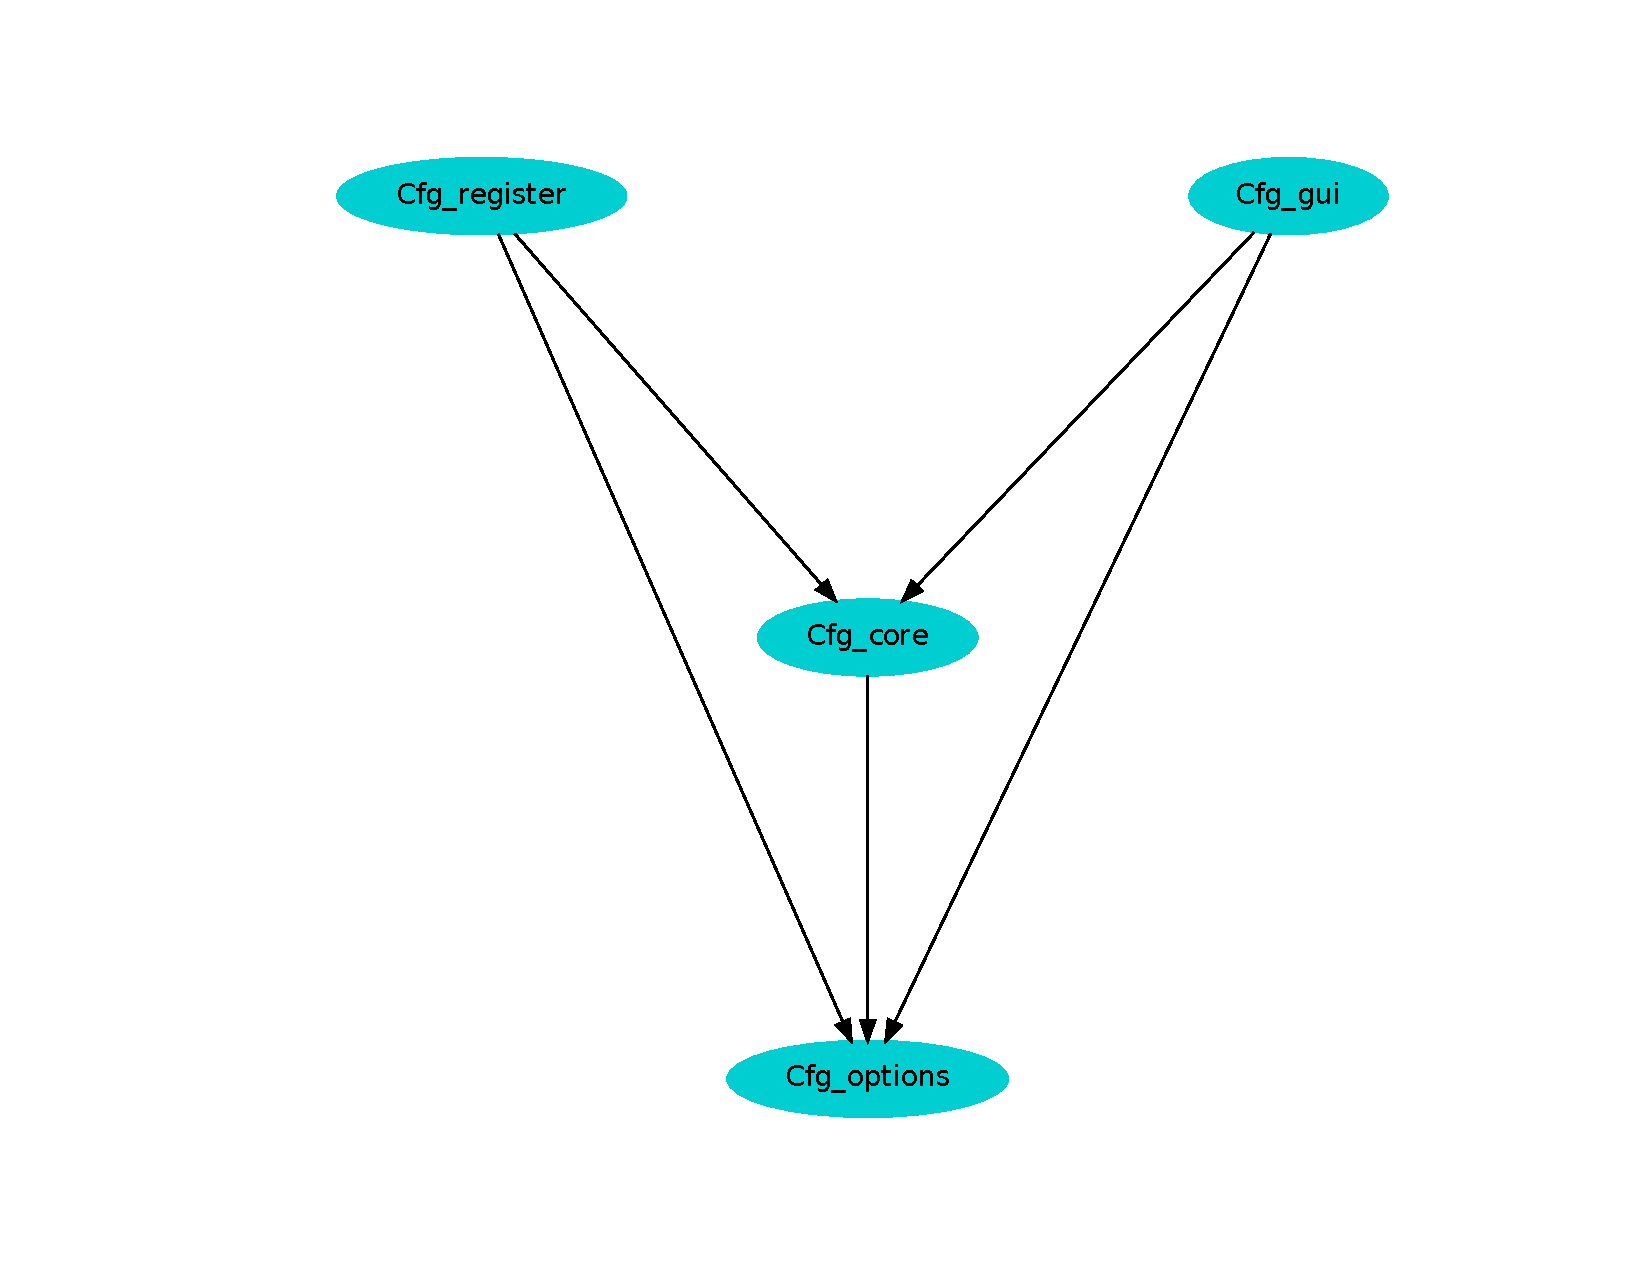
\includegraphics[width=0.5\textwidth]{./tutorial/viewcfg/pdfs/modules.pdf}
  \caption{CFG plug-in architecture}
  \label{fig:tut:cfgarchitecture}
\end{figure}

To break recursive dependencies between \ocaml modules, it is typical
that plug-in registration is done at the bottom of the module
hierarchy, while definition of the \texttt{run} function is at the
top. The GUI is also at the top of the hierarchy: the \framac
\texttt{Makefile} requires that normal plug-in modules do not depend on
GUI modules. Note that currently, the dependency from
\texttt{Cfg\_core} and \texttt{Cfg\_gui} to \texttt{Cfg\_register} is
artificial, but in future evolutions the GUI could depend on
configuration options.

\listingname{Makefile}
\codeidx{Makefile.dynamic}
\codeidx{FRAMAC\_SHARE}
\codeidx{PLUGIN\_CMO}
\codeidx{PLUGIN\_GUI\_CMO}
\codeidx{PLUGIN\_NAME}
\makefileinput{./tutorial/viewcfg/generated/split/Makefile}

In the \texttt{Makefile}, the \texttt{PLUGIN\_CMO} variable must
contain the list of file names of the ml files, in the correct \ocaml
build order. Modules in \texttt{PLUGIN\_CMO} must not depend on modules in
\texttt{PLUGIN\_GUI\_CMO}.

We also need to add an interface for the whole plug-in:
\listingname{ViewCfg.mli}
\ocamlinput{./tutorial/viewcfg/generated/split/ViewCfg.mli}

Here is the listing for the different modules:

\listingname{cfg\_options.ml}
\ocamlinput{./tutorial/viewcfg/generated/split/cfg_options.ml}

\listingname{cfg\_core.ml}
\ocamlinput{./tutorial/viewcfg/generated/split/cfg_core.ml}

\listingname{cfg\_register.ml}
\ocamlinput{./tutorial/viewcfg/generated/split/cfg_register.ml}

\listingname{cfg\_gui.ml}
\ocamlinput{./tutorial/viewcfg/generated/split/cfg_gui.ml}

\subsection{Getting your Plug-in Usable by Others}\label{tut2:api}
\index{Plug-in!API}
\todo

% TODO: A script that uses "dump_function" of the CFG plug-in

\subsection{Writing your Plug-in into the Journal}\label{tut2:journal}
\index{Journalization}
\todo

% TODO: Journalize dump_function.

% La journalisation, c'est le fait d'avoir la GUI rajouter des entrees
% dans le journal, pour pouvoir les rejouer. Ca permet, quand on
% paufine des analyses, de refaire ce qu'on a fait dans la gui
% automatiquement; apres on peut utiliser load-script pour rejouer le
% journal.

% Pour journaliser, il faut enregister la fonction pour qu'elle soit
% accessible de l'exterieur. Apres il y a un argument journalize qui
% permet de journaliser. Si je fais ca pour ma fonction dump_function,
% je vais recuperer une fonction dump_function_journalized; et c'est
% celle ci-qu'il faudrait que j'utilise dans la GUI; comme ca a chaque
% fois que je fais un "show-cfg", ce serait enregistre. La ce n'est
% pas tres interessant parce que je ne fais pas de modification de
% l'AST, mais dans le cas general ca l'est.

\subsection{Writing a Configure Script}\label{tut2:configure}
\index{Plug-in!Configure}
\todo

% Detect \dottool at compile time.
% Link to section 5.3: plug-in specific configure.in

\subsection{Getting your plug-in Usable in a Multi Projects Setting}
\label{tut2:project-and-state}
\index{Project}

\subsubsection{Registering and using state}

In this section, we will learn how to register state into \framac. A
\emph{state} is a piece of information kept by a plug-in. For instance,
the \texttt{value} plug-in computes, for each statement, a table associating to
each AST's variable a set of values the program may have at runtime: this
association table is a state.

State registration provides several features:
\begin{itemize}
\item It allows the state to be saved and reloaded with the rest of
  the session, for instance when using \texttt{frama-c -save/frama-c
    -load};
\item It helps maintaining consistency between the AST and the results and
  parameters of the analysis of the different plug-ins.
\end{itemize}

In this tutorial, we will store the file representing the \dottool
output of the control flow graph of a function (as needed by
\texttt{dump\_function}) as a string, by using a hashtable from \texttt{fundec}
to \texttt{string}. Storing this string will allow us to memoize~\cite{michie68}
our computation: the string is computed the first time the CFG of a
function is displayed, while the following requests will reuse the result of
the computation. Registering the hashtable as a \framac state is
\emph{mandatory} to ensure \framac consistency: for instance, by using a
standard \caml hashtable, a user that would have loaded several session through
the GUI could observe the CFG of function of a previous session instead of the
one he wants to observe.

Registering a state is done by a functor application:

\ocamlinput{./tutorial/viewcfg/src/register_cfg_graph_state.ml}
\scodeidx{State\_builder}{Hashtbl}
\sscodeidx{Cil\_datatype}{Fundec}{Hashtbl}
\scodeidx{Datatype}{String}
\scodeidx{Ast}{self}
\sscodeidx{Db}{Value}{self}

The \texttt{State\_builder} module provides several functors that help
registering states. \texttt{State\_builder.Hashtbl} allows the developer to
create a hashtable. It is parameterized by a module describing the hashtable
and its key, a module describing the data associated to keys, and
other informations. 

The \texttt{Datatype} and \texttt{Cil\_datatype} modules describe the
hashtable and its associated data, and explain for instance how the
datatype should be copied, printed, or marshalled to the disk. They
are part of the \texttt{Type} library~\cite{signoles:jfla11}, described in
Section~\ref{adv:datatype}. \texttt{Datatype} provides
descriptions for standard \caml types, and \texttt{Cil\_datatype} for
the CIL types (in the \texttt{Cil\_types} module).

The last module argument describes the initial size of the hashtable, a name
(mainly used for internal debugging), and a list of \emph{dependencies}. Here we
expressed that our hashtable depends on the Ast and the results of the
\texttt{Value} plug-in. For instance, whenever the \framac kernel updates one of these
states, it will automatically reset our hashtable. This ensures consistency of
the analysis: if the Ast of a function changes, or the value analysis is
executed with a different entry point, this potentially affects the display of
the control flow graph, that we must recompute.

Once the module has been declared, it is fairly easy to use it.

\ocamlinput{./tutorial/viewcfg/src/dump_to_string_memoized.ml}
\scodeidx{Visitor}{visitFramacFunction}
\ocamlinput{./tutorial/viewcfg/src/dump_function_memo_no_clear_cache.ml}

\texttt{dump\_function} now takes two steps: first the CFG is printed
to a string, then the string is printed to the \texttt{fmt}
argument. This allows the \texttt{dump\_to\_string} part to be
\emph{memoized}, \ie the results of \texttt{dump\_to\_string} are
saved so that later calls to \texttt{dump\_function} with the same
\texttt{fundec} argument reuse that result. 

If you launch \texttt{frama-c-gui} with the above code, click on
functions to view their CFG, and inspect the console, you will observe
that the string ``Computing CFG for function ...'' is displayed only
once per function.

One can see the effects of the dependency on the \texttt{Value} plug-in
by first launching the value analysis, inspecting the CFG for the
\texttt{f} function, then changing the entry point to \texttt{f} in the
CFG and re-running the value analysis. The console indicates that the
\texttt{CFG} have been recomputed. Indeed the state of the
\texttt{Value} plug-in, and of its dependencies, was reset when the
entry point was changed.

Another way to observe how \framac automatically handles states is to display a
CFG, save the session, close and restart \framac, 
and then reload the session: the control flow graph is not recomputed,
which means that \framac has automatically saved the
\texttt{Cfg\_graph\_state} with the rest of the session. Everything
should also work properly when loading several sessions.

\subsubsection{Clearing states, selection and projects}

There is one caveat though: if the user computes the CFG before
running the \texttt{Value} analysis, and then runs \texttt{Value}, he
will not see a colored graph (unless he re-launch the \texttt{Value}
analysis with different parameters). This is because the state of the
CFG is reset when the state of \texttt{Value} is reset, not when it is
first computed.

To solve this problem, we will manually reset the
\texttt{Cfg\_graph\_state} if we detect that the \texttt{Value}
analysis has been run since the last time we computed the CFG. For
that, we have to remember the previous value of
\texttt{Db.Value.is\_computed ()}, \ie to register another state:

\ocamlinput{./tutorial/viewcfg/src/register_value_computed_state.ml}
\scodeidx{State\_builder}{Ref}
\scodeidx{Datatype}{Bool}

This new state only consists of a reference to a boolean value.

Then we just replace \texttt{dump\_function} in the code above by the
following.

\ocamlinput{./tutorial/viewcfg/src/dump_function_memo_clear_cache.ml}
\sscodeidx{Db}{Value}{is\_computed}
\scodeidx{State\_selection}{with\_dependencies}
\scodeidx{Project}{clear}

The only part that need to be explained is the notion of
\emph{selection} and \emph{project}. A selection is just a set of
states; here we selected the state \texttt{Cfg\_graph\_state} with all
its dependencies, as resetting this state would also impact states
that would depend on it (even if there is none for now). We use
\texttt{Project.clear} to reset the selection.

\subsubsection{Project explanation}

A \emph{project}~\cite{project} is a consistent version of all the \emph{states}
of \framac. \framac is multi-AST, \ie \framac plug-ins can change the AST of the
program, or perform incompatible analysis (\eg with different entry
points). Projects consistently groups a version of the AST of the program, with
the states related to this AST.

The \texttt{Project.clear} function has type :
\begin{ocamlcode}
val clear: ?selection:State_selection.t -> ?project:t -> unit -> unit  
\end{ocamlcode}
\scodeidxdef{Project}{clear}
\scodeidx{State\_selection}{t}
\scodeidx{Project}{t}

The arguments \texttt{selection} and \texttt{project} can be seen as a
coordinate system, and the function allows to clear specific versions
of specific states. By default, \framac functions act on the
\emph{current} project. The developer has to use \texttt{Project.on} or optional
arguments to act on different projects. \framac automatically handles
duplication and switch of states when duplicating or changing of
projects. This is the last benefit of state registration.

To summarize:

\begin{itemize}
\item To store results, plug-ins should register \emph{states};
\item A \emph{project} is a consistent version of all the states in
  \framac, together with a version of the AST;
\item A \emph{session} is a set of \emph{projects};
\item \framac transparently handles the versioning of states when
  changing or duplicating projects, saving and reloading sessions from
  disk, etc.
\item The version of the state in a project can change; by default
  \framac functions operate on the current project.
\item A \emph{selection} is a set of states. \emph{Dependencies} allow
  to create selections.
\item As a plug-in developer, you have to remember that is up to you to preserve
  consistency between your states and their dependencies by clearing the latter
  when the former is modified in an incompatible way. For instance, it would
  have been incorrect to not call 
  \texttt{State\_selection.with\_dependencies}
  \scodeidx{State\_selection}{with\_dependencies} in the last code snippet of
  this tutorial.
\end{itemize}

Projects are generally created using copy visitors. We encourage the reader to
experiment with multiple projects development by using them. An interesting
exercise would be to change the AST so that execution of each instruction is
logged to a file, and then re-read that file to print in the CFG how much time
each instruction has been executed. Another interesting exercise would be
to use the \texttt{apply\_once} function so that the ViewCfg plug-in is executed
only once, as explained in section~\ref{tut2:options} of this tutorial.
